\documentclass{beamer}
\usepackage[utf8]{inputenc}

\usetheme{Madrid}
\usecolortheme{default}
\usepackage{amsmath,amssymb,amsfonts,amsthm}
\usepackage{txfonts}
\usepackage{tkz-euclide}
\usepackage{listings}
\usepackage{adjustbox}
\usepackage{array}
\usepackage{tabularx}
\usepackage{gvv}
\usepackage{lmodern}
\usepackage{circuitikz}
\usepackage{tikz}
\usepackage{graphicx}

\setbeamertemplate{page number in head/foot}[totalframenumber]

\title{2.7.13}
\date{September 14, 2025}
\author{EE25BTECH11001 - Aarush Dilawri}

\begin{document}

\begin{frame}
\titlepage
\end{frame}

\begin{frame}{Question}
\textbf{Question}:\\
Given vertices $\vec{A}(-4,-5)$, $\vec{B}(-1,-6)$ , $\vec{C}(-5,7)$ and $\vec{D}(4,5)$ of a quadrilateral.  
Find the area of quadrilateral $ABCD$.
\end{frame}

\begin{frame}{Solution}
Given vertices $\vec{A}=\myvec{-4\\-5}$, $\vec{B}=\myvec{-1\\-6}$,  
$\vec{C}=\myvec{-5\\7}$, $\vec{D}=\myvec{4\\5}$.  

We split the quadrilateral into triangles $\triangle ABC$ and $\triangle ACD$  
and add them to get the answer.
\end{frame}

\begin{frame}{Area of $\triangle ABC$}
\begin{align}
\text{Area}_{ABC}
&= \tfrac{1}{2}\,\big\lVert (\vec{B}-\vec{A}) \times (\vec{C}-\vec{A}) \big\rVert = 17.5
\end{align}
\end{frame}

\begin{frame}{Area of $\triangle ACD$}
\begin{align}
\text{Area}_{ACD}
&= \tfrac{1}{2}\,\big\lVert (\vec{C}-\vec{A}) \times (\vec{D}-\vec{A}) \big\rVert = 53
\end{align}
\end{frame}

\begin{frame}{Total Area}
\begin{align}
\text{Area}_{ABCD} &= \text{Area}_{ABC} + \text{Area}_{ACD} = 70.5
\end{align}
\end{frame}

\begin{frame}{Figure}
\begin{center}
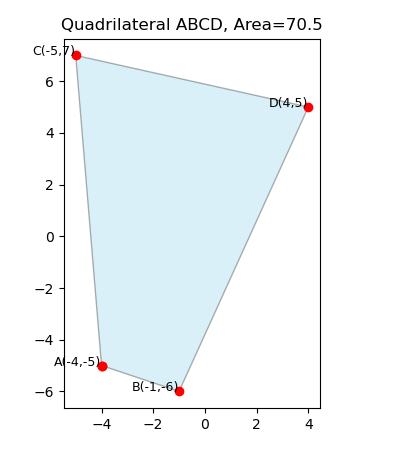
\includegraphics[width=0.6\columnwidth]{figs/fig.png}
\end{center}

\end{frame}
\begin{frame}[fragile]{C Code (code.c)}
\begin{lstlisting}[language=C]
#include <stdio.h>
#include <math.h>

double triangle_area(double x1, double y1,
                     double x2, double y2,
                     double x3, double y3) {
    return 0.5 * fabs(x1*(y2-y3) + x2*(y3-y1) + x3*(y1-y2));
}

double area_of_quadrilateral(double x1, double y1,
                             double x2, double y2,
                             double x3, double y3,
                             double x4, double y4) {
    double area1 = triangle_area(x1,y1,x2,y2,x3,y3);
    double area2 = triangle_area(x1,y1,x3,y3,x4,y4);
    return area1 + area2;
}
\end{lstlisting}
\end{frame}
\begin{frame}[fragile]{Python Code (code.py)}
\begin{lstlisting}[language=Python]
import matplotlib.pyplot as plt

def triangle_area(x1,y1,x2,y2,x3,y3):
    return 0.5 * abs(x1*(y2-y3) + x2*(y3-y1) + x3*(y1-y2))

x1, y1 = -4, -5  # A
x2, y2 = -1, -6  # B
x3, y3 = -5, 7   # C
x4, y4 = 4, 5    # D

area = triangle_area(x1,y1,x2,y2,x3,y3) + triangle_area(x1,y1,x3,y3,x4,y4)
print("Area:", area)

xs = [x1, x2, x3, x4, x1]
ys = [y1, y2, y3, y4, y1]
\end{lstlisting}
\end{frame}
\begin{frame}[fragile]{Python Code (code.py)}
\begin{lstlisting}[language=Python]
plt.fill(xs, ys, alpha=0.3, edgecolor='black')
plt.scatter([x1,x2,x3,x4],[y1,y2,y3,y4],color='red')

points = {"A": (x1,y1), "B": (x2,y2), "C": (x3,y3), "D": (x4,y4)}
for p, (x, y) in points.items():
    plt.text(x, y, f"{p}{(x,y)}")

plt.title(f"Quadrilateral ABCD, Area={area}")
plt.show()
\end{lstlisting}
\end{frame}
\begin{frame}[fragile]{Python Code (nativecode.py)}
\begin{lstlisting}[language=Python]
import ctypes
import matplotlib.pyplot as plt

lib = ctypes.CDLL("./code.so")
lib.area_of_quadrilateral.argtypes = [ctypes.c_double, ctypes.c_double,
                                      ctypes.c_double, ctypes.c_double,
                                      ctypes.c_double, ctypes.c_double,
                                      ctypes.c_double, ctypes.c_double]
lib.area_of_quadrilateral.restype = ctypes.c_double
x1, y1 = -4, -5  # A
x2, y2 = -1, -6  # B
x3, y3 = -5, 7   # C
x4, y4 = 4, 5    # D
area = lib.area_of_quadrilateral(x1,y1,x2,y2,x3,y3,x4,y4)
print("Area:", area)
\end{lstlisting}
\end{frame}
\begin{frame}[fragile]{Python Code (nativecode.py)}
\begin{lstlisting}[language=Python]
xs = [x1, x2, x3, x4, x1]
ys = [y1, y2, y3, y4, y1]

plt.fill(xs, ys, alpha=0.3, edgecolor='black')
plt.scatter([x1,x2,x3,x4],[y1,y2,y3,y4],color='red')

points = {"A": (x1,y1), "B": (x2,y2), "C": (x3,y3), "D": (x4,y4)}
for p, (x, y) in points.items():
    plt.text(x, y, f"{p}{(x,y)}")

plt.title(f"Quadrilateral ABCD, Area={area}")
plt.show()
\end{lstlisting}
\end{frame}
\end{document}
